\chapter{Data}

\section{Grammatical inflection data}

\begin{figure}[t]
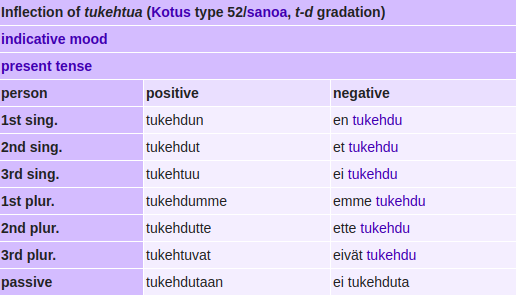
\includegraphics[width=12cm]{images/tukehtua.png}
\centering
\caption{The English Wiktionary partial inflection table for the Finnish word \textit{tukehtua}.}
\end{figure}

\begin{figure}[t]
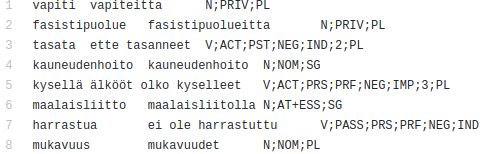
\includegraphics[width=12cm]{images/sigmorphon2018_fn.png}
\centering
\caption{A sample of the SIGMORPHON 2018 data for Finnish, scraped from Wiktionary and provided on GitHub (https://github.com/sigmorphon/conll2018/blob/master/task1/all/finnish-train-high).}
\end{figure}

I will be using the data set published for the SIGMORPHON first shared task 2018, which is publicly available on GitHub. It consists of triples - lemma, grammatical categories, and appropriately inflected form - for 103 languages, partitioned into training, development, and test sets. An example of some Finnish triples is shown in Figure 3.2. The training sets are further partitioned into low, medium, and high-resource sets; the low-resource training sets contain about 100 forms, medium about 1,000 forms, and high about 10,000 forms, with the sets being nested so that the smaller training sets are subsets of the larger ones. These data levels are used to simulate different resource settings, e.g., low-resource training sets represent data available for a poorly-resources language; the data levels can also be used to assess model learning curve \parencite{Cotterell2018b}.

\subsection{Language diversity}

The languages represented in the data cover a wide range of families and typological categories. Although over half of the languages are from the Indo-European family, a grouping that includes most languages of Europe, Greater Iran, and the northern part of the Indian subcontinent, one or more languages each of the Athabaskan, Kartvelian, Quechua, Semitic, Sino-Tibetan, Turkic, and Uralic families, as well as two isolates (Haida and Basque), are represented. Diverse inflection strategies are also represented, including suffixing, prefixing, infixing, ablaut, and introflexion, and long-distance processes like vowel harmony and consonant harmony \parencite{Cotterell2018b}.

\subsection{Sourcing and sampling}

The English Wiktionary, a collaborative online dictionary, has become something of a standard source of supervised morphological data. It provides full or partial inflection tables alongside lexeme definitions; the structure of tables is consistent for a given language and part of speech. An example table is given in figure 3.1. For some highly inflected languages (e.g., Navajo), Wiktionary only provides a fixed subset of forms. For some relationships between words that could be considered grammatical, it may simply offer them as separate lexical entries; for example, Russian perfect and imperfect forms are given as separate entries, as are Navajo verb forms that vary by aspect or thematic classifier \parencite{Wiktionary}.  

For most of the languages in the SIGMORPHON 2018 data, forms were gathered via scraping from Wiktionary. Multiple parts of speech are represented for most languages, but only parts of speech with a significant number of entries relative to all entries in a given language. Inflected forms were sampled for inclusion according to their estimated distribution in the text of Wikipedia for each respective language. For languages with sufficient data, 12,000 forms were sampled, and from these 1,000 were randomly selected for the development set and 1,000 for the testing set; the remaining 10,000 became the high-resource training set, of which 1,000 were randomly chosen as the medium-resource set and 100 of those as the low-resource set. For languages with less available data, sets might be smaller and the high-resource training set might be omitted; 17 languages lack high-resource sets \parencite{Cotterell2018b}.

\subsection{Representation of morphology}

The SIGMORPHON data set uses the UniMorph format to indicate grammatical categories  \parencite{Cotterell2018b}. The UniMorph project, initially published in 2015, is a format for encoding morphological categories uniformly cross-linguistically (\cite{SylakGlassman2015}, \cite{SylakGlassman2015a}, \cite{SylakGlassman2016}).

\section{Language typology data}

I will need numerical or categorical information about the morphological typology of the languages I consider in order to assess how typological similarities impact transfer learning. 

I may be able to gather some useful typological information the World Atlas of Language Structures (WALS), a linguistic typology database, and I also plan on generating my own typological data by computationally analyzing the SIGMORPHON 2018 data. WALS provides much of the same information that 

\subsection{Features}

The typological features I'm interested in considering include inflection shape (prefixing, suffixing, infixing, introflexion), set of inflected categories and overall paradigm size by part of speech, degree of fusion, and presence of long-distance phonological processes. 

Inflection shape may be important in determining, for instance, how soft attention models choose to focus on various parts of a word, so that a model trained on a language with a particular profile of inflection shapes may be more likely to attend to the correct parts of words when readapted to model a language with similar inflection shapes. 

Languages with similar sets of inflectional categories, e.g., languages which both mark adjectives for the gender and number of their head noun, or verbs with similar sets of tenses, may similarly benefit from transfer learning between them due to some form of model similarity. 

Fusion refers to the marking of multiple categories at once with a single indivisible morpheme, e.g., the Spanish verb \textit{hablé} "I spoke" marks tense and subject person and number with the suffix \textit{-é}, lacking separable morphemes to indicate the preterite tense and first person singular subject (cf. \textit{hablo} "I speak", \textit{habló} "he/she spoke"). Transfer learning may be beneficial between languages that both exhibit or lack fusion, or more specifically between languages that exhibit fusion between the same categories; since fusion operates over combinations of two or more categories, though, the space of possible fusion behaviors is quite large and it may be difficult to find unrelated languages with similar fusion behavior. 

Long-distance phonological processes are those by which the surface form of an affix depends on the phonological properties of a segment at some distance from the affixation site; consider my earlier example of vowel harmony in Finnish: the nouns \textit{puku} "suit" and \textit{kenkä} "shoe" have the inessive singular forms \textit{puvussa} "in the suit" and \textit{kengässä} "in the shoe", respectively, with final vowel of the suffix dependent on the set of vowels in the rest of the word. Given that long-distance processes present considerable difficulty for non-neural morphology models, neural models may have to be intensively trained to attend to such processes, presenting an opportunity for transfer learning to leverage existing knowledge.

I'd also like to take into account a more fine-grained measure of language relatedness, so that incidental typological similarities can be successfully statistically blocked against similarities arising from common origin. Two possible strategies are using detailed language genealogical trees and counting degrees of separation between languages, or finding some way to assess lexical similarity, the proportion of words between two languages which have both similar forms and meanings due to shared origin. Lexical similarity may be a more relevant measure - if word stems are similar between two languages, it is likely that grammatical affixes are as well. However, lexical similarity may also be due to shared areal loanwords, such as the profusion of Arabic loanwords into Turkish, Persian, and Urdu. Areal effects can also cause grammatical similarity to spontaneously arise between geographically collocated languages \parencite{Ponti2018}, though grammatical similarities due to shared ancestry are probably stronger. Ultimately, lexical similarity and genealogical closeness measure different types of linguistic relationships, and both should be taken into account if good data is obtainable.

Consistent and quite fine-grained information about language genealogy can be found on Ethnologue, a database of basic typological and socioliguistic information about all recognized languages \parencite{Ethnologue}. Finding good data about lexical similarity looks to be significantly more challenging - certainly, no database exists of pairwise lexical similarity between all languages, and automatically calculating lexical similarity from the SIGMORPHON 2018 data would require semantic or translation information about the words, to identify cognate words with corresponding meanings between languages. Such information may be obtainable via the Google Cloud Translation API. An easier mode of estimation may be via the "Translations" tab of entries on English Wiktionary, which provides translations of a word into a potentially large number of other languages. Average Levenshtein distance between translations for entries into a pair of languages might be a good indicator of overall lexical distance - such a method could be attempted on pairs of languages with known lexical distance to assess its utility.

\subsection{WALS}

\begin{figure}[t]
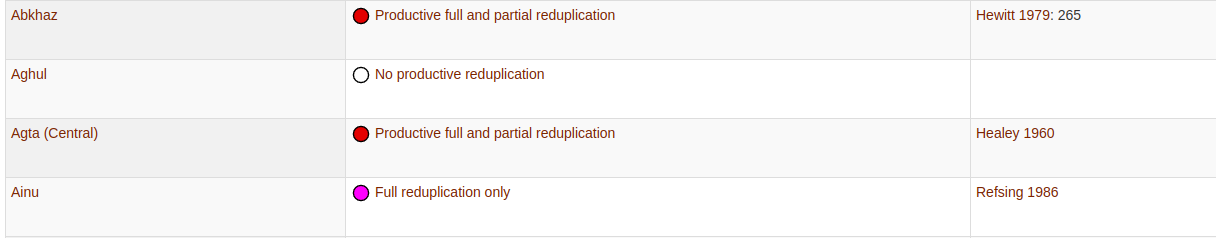
\includegraphics[width=13.5cm]{images/WALS.png}
\centering
\caption{A sample of WALS data on reduplication, available at https://wals.info/feature/27A, accessed 19 Nov 2019.}
\end{figure}

The World Atlas of Language Structures is "a large database of structural (phonological, grammatical, lexical) properties of languages gathered from descriptive materials (such as reference grammars) by a team of 55 authors." It contains information about twelve morphology features, such as "Reduplication," "Prefixing vs. Suffixing in Inflectional Morphology," and "Inflectional Synthesis of the Verb" \parencite{WALS}. Some of these may be measurable via analysis of the SIGMORPHON data as well, e.g., "Exponence of Tense-Aspect-Mood Inflection," "Prefixing vs. Suffixing in Inflectional Morphology," and "Case Syncretism," while others, such as "Reduplication" and "Locus of Marking in the Clause" would probably be harder to measure in such a way. For the features which can also be generated by looking at the SIGMORPHON data, the WALS data can at least be used as a gold standard to calibrate and assess the quality of generated metrics. WALS will not be useful in assessing overlap between sets of inflectional categories which are present or exhibit fusion in languages - its categorical tagging is simply not granular enough - but fortunately these will be relatively straightforward measures to generate from the SIGMORPHON 2018 data.

\subsection{Generated metrics}

Assessing set of inflectional categories and paradigm size based on the SIGMORPHON 2018 data will be very straightforward - I will simply need to list which UniMorph tags appear, and count the total number of UniMorph tag combinations seen, in each part of speech in each language.

To generate the other metrics, string alignment and transduction methods adopted from pre-neural morphology models will be necessary. Most clear is that to assess inflection shape, I will need to perform character alignment as in Figure 2.2 and count how many string changes take place before, after, or within the stem. 

To measure fusion between a pair of grammatical categories, average Levenshtein or LCS distance can be taken between forms that differ along both categories and compared to distance between forms that only differ along one category. For example, recall the Spanish verbs \textit{hablé} "I spoke", \textit{hablo} "I speak", \textit{habló} "he/she spoke". \textit{Hablé} differs from each of the other forms along one category - it has a different tense from \textit{hablo} and a different subject person than \textit{habló} - and its LCS distance from each is 2. \textit{Hablo} and \textit{habló} differ in both tense and subject person but also have a LCS distance of 2; the fact that forms that differ along both categories are no more dissimilar than forms that differ along one is an indicator of the fact that tense and subject agreement are fused in Spanish verbs. In contrast, consider the Finnish verbs \textit{puhuin} "I spoke", \textit{puhun} "I speak", and \textit{puhui} "he/she spoke" - \textit{puhuin} has an LCS distance of 1 from both other forms while they have an LCS distance of 2 from one another, indicating that in this case Finnish does not fuse tense and subject marking - past tense is constructed with a suffix \textit{-i} and first person subject with a subsequent suffix \textit{-n}.

Presence of long-distance phonological processes will be the most difficult to measure by analyzing the SIGMORPHON data. Fortunately, the presence of vowel and consonant harmony is typically quite binary and pervasive throughout a language's morphology, so rather than attempting to generate a measurement of it I may simply hand-annotate languages with a binary indication of whether or not they possess some long-distance process, and perhaps secondarily with a more specific indication of the type (e.g., frontness vowel harmony, sibilant harmony, etc.).